% =============================================================
%  Adaptive Multigrid Finite State Projection for the
%  Reaction-Diffusion Master Equation
%
%  Draft writeup — target: SIAM Copper Mountain Multigrid
%  Conference and SIAM Multiscale Modeling & Simulation
% =============================================================
\documentclass[review,onefignum,onetabnum]{siamart171218}

\usepackage{amsmath,amssymb,bm}
\usepackage{amsfonts}
\usepackage{mathtools}
\usepackage{algorithm}
\usepackage{algorithmic}
\usepackage{tikz}
\usepackage{enumerate}
\usepackage{graphicx}
\usepackage{subcaption}
\graphicspath{{figures/}}

% ---- theorem environments (SIAM style) ----
% theorem, lemma, corollary, definition, proposition, proof
% are already defined by siamart171218
\newsiamremark{remark}{Remark}
\newsiamremark{example}{Example}

% ---- notation shorthands ----
\newcommand{\bx}{\mathbf{x}}
\newcommand{\by}{\mathbf{y}}
\newcommand{\bz}{\mathbf{z}}
\newcommand{\bnu}{\boldsymbol{\nu}}
\newcommand{\R}{\mathbb{R}}
\newcommand{\Z}{\mathbb{Z}}
\newcommand{\Znn}{\mathbb{Z}_{\geq 0}}
\newcommand{\calX}{\mathcal{X}}
\newcommand{\calR}{\mathcal{R}}
\newcommand{\calP}{\mathcal{P}}
\newcommand{\calA}{\mathcal{A}}
\newcommand{\calF}{\mathcal{F}}
\newcommand{\calS}{\mathcal{S}}
\newcommand{\calH}{\mathcal{H}}
\newcommand{\calE}{\mathcal{E}}
\newcommand{\norm}[1]{\left\|#1\right\|}
\newcommand{\abs}[1]{\left|#1\right|}
\newcommand{\floor}[1]{\lfloor #1 \rfloor}
\newcommand{\ceil}[1]{\lceil #1 \rceil}
\newcommand{\inner}[2]{\langle #1,\, #2 \rangle}
\newcommand{\E}{\mathbb{E}}
\newcommand{\diag}{\operatorname{diag}}
\newcommand{\Tr}{\operatorname{Tr}}
\newcommand{\spn}{\operatorname{span}}
\newcommand{\Bin}{\operatorname{Bin}}
\newcommand{\Pois}{\operatorname{Pois}}
\newcommand{\TV}{\operatorname{TV}}

\title{Adaptive Multigrid Finite State Projection for the
  Reaction-Diffusion Master Equation}

\author{
  Aditya Dhumuntarao\thanks{%
    University of Colorado Boulder.
    (\email{aditya.dhumuntarao@colorado.edu}).}
}

\headers{Multigrid FSP for RDME}{Dhumuntarao}

\begin{document}

\maketitle

% =============================================================
\begin{abstract}
We develop an adaptive multigrid method for the Finite State
Projection (FSP) of the Reaction-Diffusion Master Equation
(RDME), grounded in a unified theory of \emph{spatial lumpability}
for continuous-time Markov chains.  The RDME state space
$\Znn^{N \times K}$ has two distinct hierarchical dimensions:
molecule counts (the conventional CME dimension) and spatial
position (voxel indices).  We show that coarsening the spatial
dimension by merging adjacent voxels is precisely a
Kemeny--Snell lumpability operation in the voxel-index
dimension of the Markov chain, with the lumpability parameter
$\epsilon = d_{\mathrm{inter}} / d_{\mathrm{intra}}$ playing
the role of the timescale ratio.  This unifies spatial
coarsening with quasi-steady-state (QSS) aggregation of
molecular-count states under a single framework: both are
instances of collapsing a slow region of the Markov chain
graph into a single macro-state.  The within-lump stationary
distribution --- the prolongation operator --- is a binomial
(or multinomial) distribution, available in closed form from
the fast intra-voxel diffusion process.
We prove that the projected (coarse-level) generator is exact
for linear reaction networks and characterize the closure error
for nonlinear networks.  An adaptive refinement criterion
distinguishes two failure modes of the raw flux criterion:
background inactivity (few molecules, any diffusion rate) and
structural bottlenecks (molecules present, high per-molecule
spatial flux), mirroring the bottleneck-state protection of the
companion FP-FSP algorithm for the ordinary CME.
We demonstrate the approach on a 1D birth-death-diffusion
system with an analytical reference and on the spatial
Schl\"{o}gl model, whose bistability drives stochastic
traveling fronts that the adaptive hierarchy tracks automatically.
\end{abstract}

\begin{keywords}
  reaction-diffusion master equation, finite state projection,
  multigrid, Markov chain lumpability, stochastic spatiotemporal
  dynamics, adaptive refinement, tensor product, operator splitting
\end{keywords}

% =============================================================
\section{Introduction}
\label{sec:intro}
% =============================================================

Stochastic effects are essential in biological and chemical
systems when molecular copy numbers are small or when spatial
heterogeneity drives dynamic behavior that mean-field
descriptions cannot capture \cite{Gillespie1977}.  The Chemical
Master Equation (CME) provides an exact probability-level
description of spatially homogeneous stochastic kinetics, while
its spatial generalization---the Reaction-Diffusion Master
Equation (RDME)---additionally resolves spatial gradients by
discretizing the physical domain into voxels and treating
diffusion as a jump process between adjacent voxels
\cite{Erban2009}.

The Finite State Projection (FSP) \cite{Munsky2006} truncates the
infinite state space to a finite active set $\mathcal{S}$ and
approximates the CME/RDME solution by solving the resulting
finite-dimensional linear ODE.  For the ordinary CME the state
space is $\Znn^N$ (molecule counts of $N$ species); for the RDME
on $K$ voxels it expands to $\Znn^{N \times K}$, growing
exponentially in $K$.  Even modest spatial discretizations
($K = 8$--$32$ voxels in 1D, $K = 4 \times 4$ in 2D) push the
FSP state-space to sizes that make direct computation
infeasible.

Multigrid methods \cite{Briggs2000,Trottenberg2001} achieve
algorithmic efficiency for elliptic PDEs by exploiting a
resolution hierarchy: high-frequency errors are smoothed cheaply
on the fine grid, low-frequency errors are corrected on coarse
grids.  For the RDME, the analogous hierarchy lives not in
physical space alone, but in the product structure of the full
Markov chain.

The key observation motivating this work is the following.
The RDME state space $\Znn^{N \times K}$ has two hierarchical
dimensions: (i) molecule counts, along which QSS and
aggregation methods \cite{peles,CAO20083472} coarsen fast-species
chains into macro-states; and (ii) spatial position, along which
the present work proposes to coarsen fast-diffusion voxel pairs
into coarse voxels.  Both operations are instances of the same
mathematical construction: \emph{Kemeny--Snell lumpability}
\cite{kemeny_snell_1960} applied to a continuous-time Markov chain.
A group of states is lumpable when its internal transitions are
fast relative to its exit rate; the slow chain connecting
macro-states then drives the coarse-level dynamics, while the
within-group distribution relaxes to a computable stationary
form.  For molecule-count aggregation, this within-group
distribution is a conditional quasi-stationary distribution; for
spatial coarsening, it is a binomial distribution arising from
the fast intra-voxel random walk.

This paper develops the spatial lumpability theory for the RDME,
connects it to the companion flux-based FSP work
\cite{Dhumuntarao2024}, and assembles both into a unified
adaptive framework.

\paragraph{Main contributions.}
\begin{enumerate}
  \item A \emph{spatial lumpability theory} for the RDME: we
    show that voxel merging is Kemeny--Snell lumpability in the
    spatial dimension of the RDME Markov chain, derive the
    lumpability parameter $\epsilon = d_{\mathrm{inter}} /
    d_{\mathrm{intra}}$, and prove that the prolongation
    operator is the binomial within-group stationary distribution
    (Section~\ref{sec:lumpability}).
  \item A \emph{unified coarsening table} (Table~\ref{tab:iso})
    placing spatial coarsening and molecular-count aggregation as
    two instances of the same lumpability operation on the RDME
    product state space.
  \item A coarse-level RDME generator whose consistency with the
    fine-level generator is proved for linear networks and
    characterized for nonlinear networks
    (Section~\ref{sec:coarse-gen}).
  \item A multigrid V-cycle combining operator splitting with
    FSP solves at each level (Section~\ref{sec:vcycle}).
  \item A corrected adaptive refinement criterion that
    distinguishes \emph{background inactivity} from
    \emph{spatial bottlenecks} via per-molecule flux, directly
    mirroring the bottleneck-state protection of FP-FSP
    (Section~\ref{sec:adaptive}).
\end{enumerate}

\paragraph{Related work.}
Multiscale and model-reduction methods for the CME include
quasi-steady-state (QSS) approximations
\cite{peles,CAO20083472,Cao2016} and tensor-train decompositions
\cite{Kazeev2014}.  Markov chain lumpability was characterized
classically by Kemeny and Snell \cite{kemeny_snell_1960} and by
Buchholz \cite{Buchholz1994}; approximate lumpability for
nearly-decomposable systems is studied in \cite{Simon1961}.
Spatial adaptivity for the RDME has been explored via
next-subvolume methods \cite{Elf2004} and hybrid
particle-continuum schemes.  Algebraic multigrid (AMG) has been
applied to the Fokker--Planck equation (the diffusion limit of
the CME) \cite{Dolgov2012}, but to our knowledge no multigrid or
lumpability-based method exists for the RDME at the exact
master-equation level.

% =============================================================
\section{The Reaction-Diffusion Master Equation}
\label{sec:rdme}
% =============================================================

\subsection{Setup}
\label{sec:setup}

Let $\Omega \subset \R^d$ be a bounded spatial domain partitioned
into $K$ non-overlapping voxels $\Omega_1,\ldots,\Omega_K$ of
equal volume $|\Omega_k| = V$.  Let $N$ chemical species
$S_1,\ldots,S_N$ participate in $M$ reactions and diffuse with
coefficients $D_1,\ldots,D_N$.

\begin{definition}[RDME state]
  The \emph{RDME state} is the matrix
  $\bx = (x_{ik}) \in \Znn^{N \times K}$, where $x_{ik}$ denotes
  the number of molecules of species $S_i$ in voxel $\Omega_k$.
  The full state space is $\calX = \Znn^{N \times K}$.
\end{definition}

We write $\bx_k = (x_{1k},\ldots,x_{Nk})^\top \in \Znn^N$ for
the local state in voxel $k$.  The probability distribution
$p(\bx, t) = \Pr[\mathbf{X}(t) = \bx]$ satisfies the RDME
\begin{equation}
  \label{eq:rdme}
  \frac{dp}{dt} = A_{\mathrm{RDME}}\, p,
  \quad p(\cdot,0) = p_0,
\end{equation}
where the RDME generator decomposes as
\begin{equation}
  \label{eq:gen-split}
  A_{\mathrm{RDME}} = \underbrace{\sum_{k=1}^{K} A_{\mathrm{rxn}}^{(k)}}_{\text{reactions}}
    + \underbrace{\sum_{k=1}^{K}\sum_{k' \sim k} A_{\mathrm{diff}}^{(kk')}}_{\text{diffusion}}.
\end{equation}

\subsection{Reaction and Diffusion Operators}

\paragraph{Reactions.}
For reaction $r$ with stoichiometric vector $\bnu_r \in \Z^N$
and propensity $\alpha_r : \Znn^N \to \R_{\geq 0}$, the
\emph{reaction operator} in voxel $k$ acts on probability
distributions as
\begin{equation}
  \label{eq:rxn-op}
  (A_{\mathrm{rxn}}^{(k)} p)(\bx)
  = \sum_{r=1}^{M}
    \Bigl[
      \alpha_r(\bx_k - \bnu_r)\, p(\bx - \bnu_r \mathbf{e}_k)
      - \alpha_r(\bx_k)\, p(\bx)
    \Bigr],
\end{equation}
where $\mathbf{e}_k$ denotes increment in the $k$-th voxel block,
and we set $\alpha_r(\bx_k) = 0$ if any component of $\bx_k$ is
negative.

\paragraph{Diffusion.}
Diffusion of species $S_i$ across the boundary shared by adjacent
voxels $k$ and $k'$ is modeled as a first-order jump at rate
\begin{equation}
  \label{eq:diff-rate}
  d_i^{(kk')} = \frac{D_i}{h^2},
\end{equation}
where $h = |\Omega_k|^{1/d}$ is the voxel side length.  The
\emph{diffusion operator} for the $k \to k'$ jump of species $S_i$
is
\begin{equation}
  \label{eq:diff-op}
  (A_{\mathrm{diff},i}^{(kk')} p)(\bx)
  = d_i^{(kk')}
    \bigl[
      (x_{ik}+1)\, p(\bx + \mathbf{e}_{ik} - \mathbf{e}_{ik'})
      - x_{ik}\, p(\bx)
    \bigr],
\end{equation}
and $A_{\mathrm{diff}}^{(kk')} = \sum_{i=1}^{N} A_{\mathrm{diff},i}^{(kk')}$.

\subsection{Tensor-Product Structure}
\label{sec:tensor}

The RDME state space has a natural tensor-product factorization:
\begin{equation}
  \label{eq:tensor-decomp}
  \calX = \calX_1 \otimes \calX_2 \otimes \cdots \otimes \calX_K,
  \quad \calX_k = \Znn^N.
\end{equation}
Correspondingly, any probability distribution on $\calX$ can be
viewed as a $K$-index tensor.  The diffusion operator between
voxels $k$ and $k'$ acts only on the $(k, k')$ index pair:
\begin{equation}
  A_{\mathrm{diff},i}^{(kk')}
  = I_{\calX_1} \otimes \cdots \otimes B_i^{(kk')} \otimes \cdots
    \otimes I_{\calX_K},
\end{equation}
where $B_i^{(kk')}$ is the generator of the two-site random walk
for species $S_i$ between sites $k$ and $k'$.  The reaction
operator in voxel $k$ acts only on the $k$-th tensor index.  This
Kronecker structure is fundamental to the multigrid coarsening
described in Section~\ref{sec:hierarchy}.

\subsection{Finite State Projection}

The FSP \cite{Munsky2006} restricts \eqref{eq:rdme} to a finite
active set $\calS \subset \calX$.  The \emph{FSP generator}
$A_{\calS}$ is the submatrix of $A_{\mathrm{RDME}}$ indexed by
$\calS$, with the diagonal adjusted so that any probability flux
leaving $\calS$ is absorbed:
\begin{equation}
  (A_{\calS})_{jj} = -\sum_{\bx' \notin \calS} A_{\bx j},
  \quad j \in \calS.
\end{equation}
The FSP solution $p_{\calS}(t)$ satisfies
$\norm{p(\cdot,t) - p_{\calS}(\cdot,t)}_1 \leq \epsilon_{\mathrm{FSP}}$
provided $\calS$ is chosen so that the total probability flux
out of $\calS$ over $[0,T]$ does not exceed $\epsilon_{\mathrm{FSP}}$
\cite{Munsky2006}.

For the RDME with $K$ voxels, the active set $\calS$ resides in
$\Znn^{N \times K}$, and the FSP matrix $A_{\calS}$ can reach
sizes of $10^6$--$10^{12}$ even for moderate $K$.  The multigrid
approach addresses this by solving the bulk of the dynamics on
coarser (smaller) state spaces.

% =============================================================
\section{Spatial Lumpability and the Coarsening Criterion}
\label{sec:lumpability}
% =============================================================

\subsection{Markov Chain Lumpability}

We briefly recall the classical notion of lumpability for
continuous-time Markov chains (CTMCs) \cite{kemeny_snell_1960}.

\begin{definition}[Strong lumpability]
  \label{def:lumpability}
  Let $\{X(t)\}$ be a CTMC on state space $\calX$ with generator
  $A$.  A partition $\calX = \calC_1 \cup \cdots \cup \calC_m$ is
  \emph{strongly lumpable} if there exists a generator $\bar{A}$
  on $\{1,\ldots,m\}$ such that for all $i \neq j$ and all
  $x, y \in \calC_i$,
  \begin{equation}
    \label{eq:lumpcond}
    \sum_{z \in \calC_j} A_{zx} = \sum_{z \in \calC_j} A_{zy}.
  \end{equation}
  The coarse-level generator entries are $\bar{A}_{ji} =
  \sum_{z \in \calC_j} A_{zx}$ (independent of $x \in \calC_i$).
\end{definition}

Condition \eqref{eq:lumpcond} states that the total transition
rate from any state in lump $\calC_i$ to any other lump $\calC_j$
is the same for all representatives $x \in \calC_i$.  When this
holds exactly, the marginal process on $\{1,\ldots,m\}$ is itself
a CTMC.

\subsection{Spatial Lumpability of the RDME}
\label{sec:spatial-lump}

Define the \emph{spatial coarsening partition}: for a merged
pair $\{k, k'\}$ collapsed into coarse voxel $\bar{k}$, the
lump is
\begin{equation}
  \calC_{\bar{\bx}} = \bigl\{ \bx \in \calX :
    x_{i,k} + x_{i,k'} = \bar{x}_{i\bar{k}}\;\forall i \bigr\}.
\end{equation}

\begin{proposition}[RDME is not strongly lumpable]
  \label{prop:not-strongly-lumpable}
  The RDME generator $A_{\mathrm{RDME}}$ is not strongly
  lumpable with respect to the spatial coarsening partition,
  in general.
\end{proposition}

\begin{proof}
  The diffusion rate from $k$ to an external voxel $k''$
  (not in the pair) contributes $d_i^{(kk'')} x_{ik}$ to
  the exit rate from $\calC_{\bar{\bx}}$.  Two fine states
  $\bx, \bx' \in \calC_{\bar{\bx}}$ with $x_{ik} \neq x'_{ik}$
  (but $x_{ik} + x_{ik'} = x'_{ik} + x'_{ik'}$) have different
  total exit rates, violating \eqref{eq:lumpcond}.
\end{proof}

Nevertheless, the RDME is \emph{approximately} lumpable when
the within-lump dynamics are much faster than the exit rate.
To make this precise, define the \emph{lumpability parameter}
for the spatial coarsening of the pair $\{k,k'\}$ at level $\ell$:
\begin{equation}
  \label{eq:lump-param}
  \epsilon_{kk'}^{(\ell)}
  = \frac{d_i^{(\mathrm{inter},\, \ell+1)}}
         {d_i^{(\mathrm{intra},\, \ell)}}
  = \frac{D_i / (2^\ell h)^2}{D_i / (2^{\ell-1} h)^2}
  = \frac{1}{4},
\end{equation}
which for a uniform grid is a constant $1/4$ per level,
independent of position.  For \emph{heterogeneous} diffusion
coefficients $D_i = D_i(\mathbf{x})$, the lumpability parameter
varies spatially:
\begin{equation}
  \label{eq:lump-param-hetero}
  \epsilon_{kk'}^{(\ell)}
  = \frac{D_i^{(\mathrm{inter})} / h_{\mathrm{inter}}^2}
         {D_i^{(\mathrm{intra})} / h_{\mathrm{intra}}^2}.
\end{equation}
A voxel pair is \emph{lumpable at level $\ell$} when
$\epsilon_{kk'}^{(\ell)} \ll 1$.

\begin{theorem}[Approximate lumpability error]
  \label{thm:approx-lump}
  Let $p(t)$ be the exact fine-level RDME solution and
  $\bar{p}(t) = \calR^{(\ell)} p(t)$ its coarse marginal.
  Suppose the within-lump intra-voxel diffusion has spectral gap
  $\lambda_2 \geq d_{\min}$, and the inter-lump exit rate
  satisfies $\lambda_{\mathrm{exit}} \leq \lambda_{\mathrm{exit},\max}$.
  Then the coarse marginal $\bar{p}(t)$ satisfies an
  approximate RDME \eqref{eq:coarse-rdme} with error
  \begin{equation}
    \label{eq:lump-error}
    \norm{\frac{d\bar{p}}{dt} - \bar{A}^{(\ell)} \bar{p}}_1
    \leq C \cdot \epsilon_{kk'}^{(\ell)} \cdot \lambda_{\mathrm{exit},\max}
    \cdot \norm{\bar{p}}_1,
  \end{equation}
  where the lumpability parameter
  $\epsilon_{kk'}^{(\ell)} = \lambda_{\mathrm{exit},\max} / \lambda_2$.
\end{theorem}

\begin{remark}[Connection to nearly-decomposable systems]
  Theorem~\ref{thm:approx-lump} is an instance of the
  nearly-decomposable Markov chain theory of Simon and Ando
  \cite{Simon1961}: a nearly-decomposable system (strong
  intra-block coupling, weak inter-block coupling) evolves on
  two timescales, with the fast dynamics reaching a quasi-steady
  state within each block.  The RDME coarsening makes this
  precise for the spatial block structure.
\end{remark}

\subsection{The Dual Lumpability: A Unified Table}
\label{sec:dual-lump}

The RDME Markov chain admits lumpability in \emph{two}
independent dimensions of its product state space.
Table~\ref{tab:iso} presents the complete isomorphism.

\begin{table}[h]
\caption{Markov chain lumpability in the two dimensions of
  the RDME state space $\Znn^{N \times K}$.}
\label{tab:iso}
\centering
\begin{tabular}{lll}
  \hline
  & \textbf{Molecule-count dimension} & \textbf{Spatial dimension} \\
  \hline
  States / positions & $\bx_k \in \Znn^N$ & $k \in \{1,\ldots,K\}$ \\
  Transitions & reactions, rate $\alpha_r(\bx_k)$ & diffusion, rate $d_i x_{ik}$ \\
  Slow region & slow-reaction chain & slow-diffusion spatial region \\
  Coarsening & state aggregation (QSS) & voxel merging (spatial MG) \\
  Lumpability param & $\epsilon = k_{\mathrm{slow}} / k_{\mathrm{fast}}$ &
    $\epsilon = d_{\mathrm{inter}} / d_{\mathrm{intra}}$ \\
  Within-lump stationary & conditional quasi-stationary & $\mathrm{Binomial}(n, \theta)$ \\
  Bottleneck & high $\alpha_r(\bx)/p(\bx)$ & high $\Phi_{kk'}/\E[x_{ik}]$ \\
  Bottleneck action & protect from pruning \cite{Dhumuntarao2024} &
    refine (keep at fine level) \\
  \hline
\end{tabular}
\end{table}

The key structural point is that both coarsenings are driven by
the same principle: \emph{a group of states connected by fast
internal transitions collapses to a single macro-state whose
outgoing rates are determined by the within-group stationary
distribution}.  The within-group stationary distribution plays
the role of the prolongation operator in both cases.

\subsection{Two Failure Modes of the Raw Flux Criterion}
\label{sec:failure-modes}

A naive adaptive criterion might merge voxel pairs with small
\emph{total inter-voxel flux} $\Phi_{kk'} = \sum_i d_i
\E[x_{ik}]$.  This confounds two structurally distinct cases:

\begin{enumerate}
  \item \textbf{Background inactivity.}  Few molecules are
    present ($\E[x_{ik}] \approx 0$), so $\Phi_{kk'} \approx 0$
    regardless of $d_i$.  The pair is irrelevant to the dynamics
    and merging is both valid and cheap.

  \item \textbf{Structural slowness.}  Molecules are present,
    but $d_i$ is intrinsically small (e.g., a membrane region
    or narrow spatial channel).  Then $\Phi_{kk'}$ may be small
    despite $\E[x_{ik}]$ being non-negligible.  The pair is a
    \emph{spatial bottleneck}: molecules must pass through it to
    transit between spatial regions.  Merging is
    \emph{structurally invalid} if $\epsilon_{kk'} \sim O(1)$,
    and harmful if $\epsilon_{kk'} > 1$ (inter-voxel rate
    exceeds intra-voxel rate).
\end{enumerate}

Case~2 is the spatial analogue of a CME bottleneck state: in
\cite{Dhumuntarao2024}, a bottleneck state has low probability
(small $p(\bx)$) but high flux-to-probability ratio
$\alpha_r(\bx)/p(\bx)$, making it dangerous to prune.
Analogously, a spatial bottleneck voxel may have low absolute
flux $\Phi_{kk'}$ but high \emph{per-molecule flux}
$\phi_{kk'} = \Phi_{kk'} / \max(1, \sum_i \E[x_{ik}])$,
making it dangerous to merge.

% =============================================================
\section{Spatial Coarsening Hierarchy}
\label{sec:hierarchy}
% =============================================================

\subsection{Coarsening Map}
\label{sec:coarsen}

We construct a $L$-level hierarchy of voxel grids.  At level
$\ell = 0$ (finest) we have $K^{(0)} = K$ voxels.  At level
$\ell$, adjacent pairs are merged so that
$K^{(\ell)} = K^{(\ell-1)}/2$ (assuming $K$ is a power of 2 for
simplicity; non-power-of-2 and higher-dimensional cases are
discussed in Section~\ref{sec:extensions}).  We denote the voxels
at level $\ell$ by $\Omega_1^{(\ell)},\ldots,\Omega_{K^{(\ell)}}^{(\ell)}$,
with
\begin{equation}
  \Omega_j^{(\ell)} = \Omega_{2j-1}^{(\ell-1)} \cup \Omega_{2j}^{(\ell-1)},
  \quad j = 1,\ldots,K^{(\ell)}.
\end{equation}

\begin{definition}[Coarse state and state space]
  \label{def:coarse-state}
  The \emph{coarse state} at level $\ell$ is
  $\bar{\bx}^{(\ell)} = (\bar{x}_{ij}^{(\ell)}) \in \Znn^{N \times K^{(\ell)}}$,
  where
  \begin{equation}
    \label{eq:coarsen-counts}
    \bar{x}_{ij}^{(\ell)} = x_{i,2j-1}^{(\ell-1)} + x_{i,2j}^{(\ell-1)},
    \quad i=1,\ldots,N,\quad j=1,\ldots,K^{(\ell)}.
  \end{equation}
  The coarse state space is $\bar{\calX}^{(\ell)} = \Znn^{N \times K^{(\ell)}}$.
\end{definition}

The key observation is that \eqref{eq:coarsen-counts} is a
\emph{sufficient statistic} for all chemical reactions within
each coarse voxel under the well-mixed (uniform spatial
distribution) assumption, which holds exactly when intra-voxel
diffusion is fast.

\subsection{Restriction Operator}
\label{sec:restriction}

\begin{definition}[Restriction]
  \label{def:restriction}
  The \emph{restriction operator}
  $\calR^{(\ell)} : \R^{\calX^{(\ell-1)}} \to \R^{\bar{\calX}^{(\ell)}}$
  is the marginalization over all fine-level states consistent
  with a given coarse state:
  \begin{equation}
    \label{eq:restriction}
    (\calR^{(\ell)} p)(\bar{\bx})
    = \sum_{\substack{\bx \in \calX^{(\ell-1)} \\
        x_{i,2j-1}+x_{i,2j}=\bar{x}_{ij}\;\forall i,j}}
      p(\bx).
  \end{equation}
\end{definition}

The tensor-product structure \eqref{eq:tensor-decomp} implies
that $\calR^{(\ell)}$ factorizes over coarse-voxel pairs:
\begin{equation}
  \label{eq:restriction-factored}
  \calR^{(\ell)} = \bigotimes_{j=1}^{K^{(\ell)}} \calR_j^{(\ell)},
\end{equation}
where
$(\calR_j^{(\ell)} q)(\bar{\bx}_j)
  = \sum_{\bm_j : \bm_j + (\bar{\bx}_j - \bm_j) = \bar{\bx}_j} q(\bm_j,\, \bar{\bx}_j - \bm_j)$
sums over all splits of the coarse count $\bar{\bx}_j$ into the
two fine-voxel sub-counts.

\paragraph{Properties.}
$\calR^{(\ell)}$ is a stochastic map: it preserves non-negativity
and total mass, $\norm{\calR^{(\ell)} p}_1 = \norm{p}_1$.  It is
surjective but not injective; the kernel consists of distributions
that sum to zero on each fiber $\{\bx : \text{\eqref{eq:coarsen-counts} holds}\}$.

\subsection{Prolongation Operator}
\label{sec:prolongation}

To reconstruct the fine-level distribution from the coarse level,
we need a probabilistic model for the \emph{within-coarse-voxel}
distribution of molecules.  The key insight is that, under fast
intra-voxel diffusion, this distribution reaches stationarity
quickly and is available in closed form.

\begin{proposition}[Stationary within-voxel distribution]
  \label{prop:stationary-split}
  Consider the two-site random walk for species $S_i$ with $n$
  molecules distributed between fine voxels $\Omega_{2j-1}$ and
  $\Omega_{2j}$, each of volume $V$.  The jump rates are
  $d_i$ in both directions.  The stationary distribution of
  the molecule count $m$ in $\Omega_{2j-1}$ is
  \begin{equation}
    \label{eq:binomial-stat}
    \pi_i(m \mid n) = \binom{n}{m} \left(\tfrac{1}{2}\right)^n,
    \quad m = 0,1,\ldots,n.
  \end{equation}
  For voxels of unequal volumes $V_{2j-1}$ and $V_{2j}$:
  \begin{equation}
    \label{eq:binomial-stat-unequal}
    \pi_i(m \mid n) = \binom{n}{m} \theta_j^m (1-\theta_j)^{n-m},
    \quad \theta_j = \frac{V_{2j-1}}{V_{2j-1}+V_{2j}}.
  \end{equation}
\end{proposition}

\begin{proof}
  The two-site random walk generator for count $m$ in site 1
  (total $n$) is
  $B_i(m,m-1) = d_i m$ (jump to site 2) and
  $B_i(m,m+1) = d_i(n-m)$ (jump from site 2).
  Detailed balance with $\pi_i(m \mid n) \propto \binom{n}{m}$
  follows from $d_i m \cdot \pi_i(m) = d_i(n-m+1) \cdot \pi_i(m-1)$,
  which is satisfied by \eqref{eq:binomial-stat}.
\end{proof}

\begin{definition}[Prolongation]
  \label{def:prolongation}
  Assume independence across species and coarse voxels (justified
  when molecules are dilute or reactions are weak relative to
  diffusion within each coarse pair).  The
  \emph{prolongation operator}
  $\calP^{(\ell)} : \R^{\bar{\calX}^{(\ell)}} \to \R^{\calX^{(\ell-1)}}$
  is
  \begin{equation}
    \label{eq:prolongation}
    (\calP^{(\ell)} \bar{p})(\bx)
    = \bar{p}(\bar{\bx}) \cdot
      \prod_{i=1}^{N} \prod_{j=1}^{K^{(\ell)}}
      \pi_i\!\left(x_{i,2j-1} \mid x_{i,2j-1}+x_{i,2j}\right),
  \end{equation}
  where $\bar{\bx}$ is the coarse state corresponding to $\bx$
  via \eqref{eq:coarsen-counts}.
\end{definition}

\begin{proposition}[Consistency]
  \label{prop:consistency}
  $\calR^{(\ell)} \calP^{(\ell)} = I_{\bar{\calX}^{(\ell)}}$.
\end{proposition}

\begin{proof}
  For any $\bar{p}$ and $\bar{\bx}$:
  $(\calR^{(\ell)} \calP^{(\ell)} \bar{p})(\bar{\bx})
   = \bar{p}(\bar{\bx}) \sum_{\bx \mapsto \bar{\bx}}
     \prod_{i,j} \pi_i(x_{i,2j-1} \mid \bar{x}_{ij})
   = \bar{p}(\bar{\bx})$,
  since the binomial sums to 1 over all splits.
\end{proof}

The projector $\Pi^{(\ell)} = \calP^{(\ell)} \calR^{(\ell)}$ is
\emph{not} the identity on the fine level; the complementary
projector $I - \Pi^{(\ell)}$ captures the intra-voxel
fluctuations that the coarse level cannot represent.

% =============================================================
\section{The Coarse-Level Generator}
\label{sec:coarse-gen}
% =============================================================

\subsection{Construction}

Given the restriction and prolongation operators, a natural
definition of the coarse-level generator is the Petrov--Galerkin
projection
\begin{equation}
  \label{eq:coarse-gen}
  \bar{A}^{(\ell)} = \calR^{(\ell)} A_{\mathrm{RDME}} \calP^{(\ell)}.
\end{equation}

We derive $\bar{A}^{(\ell)}$ explicitly by applying it to
$\bar{A}^{(\ell)} = \calR^{(\ell)} (A_{\mathrm{rxn}} + A_{\mathrm{intra}} + A_{\mathrm{inter}}) \calP^{(\ell)}$,
where
\begin{align}
  A_{\mathrm{rxn}} &= \textstyle\sum_k A_{\mathrm{rxn}}^{(k)},\\
  A_{\mathrm{intra}} &= \textstyle\sum_j A_{\mathrm{diff}}^{(2j-1,2j)} + A_{\mathrm{diff}}^{(2j,2j-1)},\\
  A_{\mathrm{inter}} &= A_{\mathrm{RDME}} - A_{\mathrm{rxn}} - A_{\mathrm{intra}}.
\end{align}

\paragraph{Intra-voxel diffusion term.}
Since $\calP^{(\ell)}$ assigns the binomial stationary
distribution and $A_{\mathrm{intra}}$ generates the corresponding
random walk, the product $A_{\mathrm{intra}} \calP^{(\ell)}
\bar{p}$ gives the flux from this stationary state, which
integrates to zero under $\calR^{(\ell)}$:
\begin{equation}
  \label{eq:intra-zero}
  \calR^{(\ell)} A_{\mathrm{intra}} \calP^{(\ell)} = 0.
\end{equation}
The fast intra-voxel diffusion thus drops out of the
coarse-level generator---it is exactly accounted for by
the prolongation operator.

\paragraph{Inter-voxel diffusion term.}
For species $S_i$ jumping from coarse voxel $j$ to adjacent
coarse voxel $j'$ with fine-grid rate $d_i$:
\begin{equation}
  \label{eq:coarse-diff-rate}
  \bar{d}_i^{(jj')} = d_i \cdot \frac{|\partial\Omega_j^{(\ell)} \cap \partial\Omega_{j'}^{(\ell)}|}{|\partial\Omega_j^{(\ell)} \cap \partial\Omega_{j'}^{(\ell)}|_{\mathrm{fine}}}
  = \frac{D_i}{(2^{\ell}h)^2}.
\end{equation}
The coarse inter-voxel diffusion operator has the same form as
\eqref{eq:diff-op} but with rate $\bar{d}_i^{(jj')} = D_i/(2^\ell h)^2$
and coarse counts $\bar{x}_{ij}$.

\paragraph{Reaction term.}
\begin{proposition}[Exact coarsening for linear networks]
  \label{prop:linear-exact}
  If all reaction propensities are affine in the local state
  $\bx_k$ (i.e., zero-order: $\alpha_r = c_r$, or first-order:
  $\alpha_r = c_r x_{ik}$), then
  \begin{equation}
    \label{eq:linear-exact}
    \calR^{(\ell)} A_{\mathrm{rxn}}^{(2j-1)} \calP^{(\ell)}
    + \calR^{(\ell)} A_{\mathrm{rxn}}^{(2j)} \calP^{(\ell)}
    = \bar{A}_{\mathrm{rxn}}^{(j,\ell)},
  \end{equation}
  where $\bar{A}_{\mathrm{rxn}}^{(j,\ell)}$ is the reaction
  generator with propensities evaluated at the coarse count
  $\bar{\bx}_j$.
\end{proposition}

\begin{proof}
  For a zero-order reaction $\alpha_r = c_r$, both fine voxels
  contribute $c_r$ independently, so the coarse propensity is
  $2c_r$ (assuming equal volumes and rescaling by voxel count;
  see Remark~\ref{rem:volume-scaling}).  For a first-order
  reaction $\alpha_r(\bx_k) = c_r x_{ik}$, the expected total
  propensity in the coarse voxel is
  $c_r \E_\pi[x_{i,2j-1} + x_{i,2j}] = c_r \bar{x}_{ij}$,
  since the binomial mean is $n/2$ per sub-voxel.  The operator
  identity then follows by direct computation using the
  linearity of $\calR^{(\ell)}$ and $\calP^{(\ell)}$.
\end{proof}

\begin{remark}[Nonlinear closure error]
  \label{rem:closure}
  For a second-order (bimolecular) propensity
  $\alpha_r(\bx_k) = c_r x_{ik} x_{jk}$ ($i \neq j$), the
  coarsening introduces a \emph{closure error}:
  \begin{equation}
    \label{eq:closure-error}
    \E_\pi[x_{ik} x_{jk}] = \frac{\bar{x}_{ij}^{(k)} \bar{x}_{ij}^{(j)}}{4}
      + \text{covariance term}.
  \end{equation}
  For a binomial distribution on $n$ particles between two sites,
  $\E[m^2] = n/4 \cdot (1 + (n-1)/2)$ and
  $\operatorname{Var}[m] = n/4$.  The relative closure error
  for the reaction propensity is $O(1/\bar{x}_{ij})$, vanishing
  in the high-copy-number limit.
\end{remark}

\begin{remark}[Volume rescaling]
  \label{rem:volume-scaling}
  Reaction rates in the RDME use the \emph{combinatorial}
  propensity that depends on the local volume through the
  conversion factor $N_A V$ (Avogadro's number times voxel
  volume).  When two voxels of volume $V$ merge into one of
  volume $2V$, bimolecular propensities must be rescaled as
  $c_r \to c_r / 2$ to maintain the correct macroscopic rate.
  Our framework handles this by tracking voxel volumes
  $V^{(\ell)} = 2^\ell V$ at each level.
\end{remark}

\subsection{Full Coarse RDME}

Combining the results above, the coarse-level RDME at level
$\ell$ is
\begin{equation}
  \label{eq:coarse-rdme}
  \frac{d\bar{p}^{(\ell)}}{dt}
  = \bar{A}^{(\ell)} \bar{p}^{(\ell)},
  \quad
  \bar{A}^{(\ell)}
  = \sum_{j=1}^{K^{(\ell)}} \bar{A}_{\mathrm{rxn}}^{(j,\ell)}
    + \sum_{\langle j,j'\rangle} \bar{A}_{\mathrm{diff}}^{(jj',\ell)},
\end{equation}
with coarse propensities evaluated at coarse counts
$\bar{\bx}^{(\ell)}$ and diffusion rates $\bar{d}_i = D_i/(2^\ell h)^2$.
Equation \eqref{eq:coarse-rdme} is itself an RDME on a coarser
spatial grid---it has the same structural form as the fine-level
RDME, enabling recursive application of the coarsening hierarchy.

% =============================================================
\section{Multigrid V-Cycle for the RDME}
\label{sec:vcycle}
% =============================================================

\subsection{Operator Splitting}

We decompose the fine-level RDME generator as
\begin{equation}
  \label{eq:split}
  A_{\mathrm{RDME}} = A_{\mathrm{fast}} + A_{\mathrm{slow}},
\end{equation}
where
\begin{align}
  A_{\mathrm{fast}} &= A_{\mathrm{intra}}
    = \sum_{j=1}^{K^{(1)}}
      \bigl(A_{\mathrm{diff}}^{(2j-1,2j)} + A_{\mathrm{diff}}^{(2j,2j-1)}\bigr),\\
  A_{\mathrm{slow}} &= A_{\mathrm{rxn}} + A_{\mathrm{inter}}.
\end{align}
The timescale ratio is $\epsilon = \norm{A_{\mathrm{slow}}} / \norm{A_{\mathrm{fast}}} \ll 1$ under fast diffusion.

The intra-voxel diffusion generator $A_{\mathrm{fast}}$ is
block-diagonal with $K/2$ blocks, each acting on a two-site
system.  Consequently, $e^{\tau A_{\mathrm{fast}}}$ is cheap to
apply: each block is a $\binom{n_{\max}+N}{N} \times \binom{n_{\max}+N}{N}$ matrix where $n_{\max}$ is the local count
bound, and the blocks are independent.

\subsection{Two-Level V-Cycle}

\begin{algorithm}[H]
  \caption{Two-Level Multigrid V-Cycle
    $\mathbf{MG2}(p^h, t, \Delta t; \tau_{\mathrm{pre}}, \tau_{\mathrm{post}})$}
  \label{alg:vcycle}
  \begin{algorithmic}[1]
    \REQUIRE{Fine-level probability vector $p^h$ at time $t$,
      time step $\Delta t$, smoothing times $\tau_{\mathrm{pre}},
      \tau_{\mathrm{post}} > 0$}
    \ENSURE{Approximate $p^h(t+\Delta t)$}
    \STATE \textbf{Pre-smooth:}
      $\tilde{p}^h \leftarrow e^{\tau_{\mathrm{pre}} A_{\mathrm{fast}}} p^h$
      \COMMENT{Fast intra-voxel relaxation}
    \STATE \textbf{Restrict:}
      $p^{2h} \leftarrow \calR\, \tilde{p}^h$
      \COMMENT{Marginalize to coarse level}
    \STATE \textbf{Coarse solve (via FSP):}
      $\bar{p}^{2h} \leftarrow e^{\Delta t\, \bar{A}^{(1)}} p^{2h}$
      \COMMENT{Full step on coarse RDME}
    \STATE \textbf{Prolongate correction:}
      $p^h \leftarrow \tilde{p}^h + \calP\bigl(\bar{p}^{2h} - p^{2h}\bigr)$
      \COMMENT{Inject coarse-level update}
    \STATE \textbf{Post-smooth:}
      $p^h_{\mathrm{new}} \leftarrow e^{\tau_{\mathrm{post}} A_{\mathrm{fast}}} p^h$
      \COMMENT{Re-equilibrate intra-voxel}
    \STATE \textbf{Return} $p^h_{\mathrm{new}}$
  \end{algorithmic}
\end{algorithm}

\begin{remark}[Interpretation as operator splitting]
  \label{rem:splitting}
  When $\tau_{\mathrm{pre}} = \tau_{\mathrm{post}} = 0$ and the
  prolongation uses the current conditional distribution (not the
  stationary binomial), Algorithm~\ref{alg:vcycle} reduces to
  a standard Lie--Trotter splitting between $A_{\mathrm{slow}}$
  and the coarse-corrected fast dynamics.  The pre- and
  post-smoothing steps provide an order-$\tau^2$ Strang-type
  correction that improves accuracy.
\end{remark}

\subsection{Recursive Multi-Level V-Cycle}

For an $L$-level hierarchy the coarse solve in
Algorithm~\ref{alg:vcycle} is replaced by a recursive V-cycle
call (for W-cycle, by two recursive calls).

\begin{algorithm}[H]
  \caption{$L$-Level Multigrid V-Cycle
    $\mathbf{MG}(p^{(\ell)}, t, \Delta t, \ell)$}
  \label{alg:vcycle-l}
  \begin{algorithmic}[1]
    \IF{$\ell = L$ (coarsest level)}
      \STATE Solve $\bar{p}^{(L)} \leftarrow e^{\Delta t \bar{A}^{(L)}} p^{(L)}$ exactly (via FSP)
    \ELSE
      \STATE Pre-smooth: $\tilde{p}^{(\ell)} \leftarrow e^{\tau_{\mathrm{pre}} A_{\mathrm{fast}}^{(\ell)}} p^{(\ell)}$
      \STATE Restrict: $p^{(\ell+1)} \leftarrow \calR^{(\ell+1)} \tilde{p}^{(\ell)}$
      \STATE Coarse correct: $\bar{p}^{(\ell+1)} \leftarrow \mathbf{MG}(p^{(\ell+1)}, t, \Delta t, \ell+1)$
      \STATE Prolongate: $p^{(\ell)} \leftarrow \tilde{p}^{(\ell)} + \calP^{(\ell+1)}(\bar{p}^{(\ell+1)} - p^{(\ell+1)})$
      \STATE Post-smooth: $p^{(\ell)} \leftarrow e^{\tau_{\mathrm{post}} A_{\mathrm{fast}}^{(\ell)}} p^{(\ell)}$
    \ENDIF
    \STATE \textbf{Return} $p^{(\ell)}$
  \end{algorithmic}
\end{algorithm}

\subsection{Smoothing Parameter Selection}

The pre-smooth time $\tau_{\mathrm{pre}}$ should be long enough to
reduce the intra-voxel distribution to near-stationarity, but
short compared to $\Delta t$ to avoid wasting computation.  The
spectral gap of the two-site random walk generator $B_i^{(kk')}$
with $n$ particles is $\lambda_2 = 2d_i$ (independent of $n$),
giving an $\epsilon_{\mathrm{smooth}}$-relaxation time of
\begin{equation}
  \label{eq:smooth-time}
  \tau_{\mathrm{pre}} = \frac{\log(1/\epsilon_{\mathrm{smooth}})}{2d_i}.
\end{equation}
For $d_i = D_i/h^2 \gg 1$, this $\tau_{\mathrm{pre}}$ is
extremely small, justifying the approximation that pre-smoothing
is computationally negligible compared to the coarse solve.

% =============================================================
\section{Error Analysis}
\label{sec:error}
% =============================================================

\subsection{Per-Cycle Error Decomposition}

The error introduced in one V-cycle step from $t$ to $t+\Delta t$
decomposes as follows.  Let
$p_{\mathrm{exact}}^h = e^{\Delta t A_{\mathrm{RDME}}} p^h(t)$
and $p_{\mathrm{MG}}^h = \mathbf{MG2}(p^h(t), t, \Delta t)$.

\begin{theorem}[V-cycle error bound]
  \label{thm:vcycle-error}
  Suppose the intra-voxel diffusion rate satisfies
  $d_i \geq d_{\min}$ and the smoothing time is chosen as
  in \eqref{eq:smooth-time}.  Then
  \begin{equation}
    \label{eq:vcycle-error}
    \norm{p_{\mathrm{exact}}^h - p_{\mathrm{MG}}^h}_1
    \leq C_1 \epsilon_{\mathrm{smooth}}
         + C_2 \epsilon_{\mathrm{split}} \Delta t
         + C_3 \delta_{\mathrm{closure}} \Delta t
         + \epsilon_{\mathrm{FSP}},
  \end{equation}
  where
  \begin{enumerate}[(i)]
    \item $\epsilon_{\mathrm{smooth}} =
           e^{-2 d_{\min} \tau_{\mathrm{pre}}}$
           is the pre-smoothing residual;
    \item $\epsilon_{\mathrm{split}} = \norm{A_{\mathrm{fast}}}\,
           \norm{A_{\mathrm{slow}}} \Delta t$
           is the Lie--Trotter splitting error (second-order with
           Strang splitting);
    \item $\delta_{\mathrm{closure}} = O(1/n_{\min})$ is the
           closure error from nonlinear propensities
           (Remark~\ref{rem:closure});
    \item $\epsilon_{\mathrm{FSP}}$ is the FSP truncation error
          from the coarse-level solve.
  \end{enumerate}
\end{theorem}

\begin{remark}[Linear networks: exact coarsening]
  For linear reaction networks ($C_3 = 0$) and in the limit
  $\epsilon_{\mathrm{smooth}} \to 0$ (instantaneous pre-smoothing),
  the only errors are the splitting error and FSP truncation.  The
  splitting error can be made $O(\Delta t^3)$ with Strang splitting,
  recovering second-order accuracy in time.
\end{remark}

\subsection{Complexity Comparison}

Let $|\calS^{(0)}|$ denote the fine-level FSP state-space size.
Under the assumption that the coarse-level state space is
$|\calS^{(\ell)}| \approx |\calS^{(0)}| / 2^{N \ell}$ (due to
reduced per-voxel count bounds on the coarser grid), the cost of
the coarse solve is:

\begin{center}
\begin{tabular}{lcc}
  \hline
  Method & State-space size & Cost per step \\
  \hline
  Fine FSP (no MG) & $|\calS^{(0)}|$ & $O(|\calS^{(0)}|)$ \\
  Coarse solve only & $|\calS^{(L)}|$ & $O(|\calS^{(L)}|)$ \\
  $L$-level V-cycle & $|\calS^{(0)}| + \cdots + |\calS^{(L)}|$
    & $O(|\calS^{(0)}|)$ \\
  \hline
\end{tabular}
\end{center}

The overhead of the V-cycle over the fine-level solve is a
geometric series bounded by $O(|\calS^{(0)}|)$; the benefit is
that the coarse solve can use much larger time steps
$\Delta t \sim O(1/\norm{A_{\mathrm{slow}}})$ rather than the
fine-level stability limit $\Delta t \sim O(1/\norm{A_{\mathrm{fast}}})$,
which in stiff systems may be $10^2$--$10^6$ times larger.

% =============================================================
\section{Adaptive Spatial Refinement}
\label{sec:adaptive}
% =============================================================

\subsection{Two Quantites: Total Flux and Per-Molecule Flux}

We define two inter-voxel flux quantities that together determine
the refinement decision.

\begin{definition}[Inter-voxel flux quantities]
  \label{def:flux-quantities}
  For adjacent voxels $k$ and $k'$, define the
  \emph{total spatial flux}
  \begin{equation}
    \label{eq:spatial-flux}
    \Phi_{kk'} = \sum_{i=1}^{N} d_i^{(kk')}\, \E_p[x_{ik}],
  \end{equation}
  and the \emph{per-molecule spatial flux}
  \begin{equation}
    \label{eq:specific-flux}
    \phi_{kk'} = \frac{\Phi_{kk'}}{\max\!\left(1,\,
      \sum_{i=1}^N \E_p[x_{ik}]\right)}.
  \end{equation}
  The total flux $\Phi_{kk'}$ measures how much probability
  mass crosses the boundary per unit time; the per-molecule
  flux $\phi_{kk'}$ measures the average rate at which
  \emph{each molecule} crosses, i.e., the local diffusion
  conductance.
\end{definition}

\subsection{Two-Criterion Refinement Rule}
\label{sec:two-criterion}

Section~\ref{sec:failure-modes} identified two failure modes of
a naive total-flux criterion.  The corrected adaptive refinement
rule uses both quantities.

\begin{definition}[Two-criterion refinement]
  \label{def:two-criterion}
  Let $\bar{\phi} = |\{\langle k,k'\rangle\}|^{-1}
  \sum_{\langle k,k'\rangle} \phi_{kk'}$ be the mean
  per-molecule flux across all boundaries.  A voxel pair
  $\{k,k'\}$ is \emph{refined} (kept at the current fine
  level) if either
  \begin{align}
    \label{eq:lump-valid}
    \epsilon_{kk'}^{(\ell)} &\geq \epsilon_{\mathrm{lump}}
    \quad \text{(lumpability violated),} \\
    \label{eq:bottleneck}
    \phi_{kk'} &\geq \epsilon_{\mathrm{bn}} \cdot \bar{\phi}
    \quad \text{(spatial bottleneck detected).}
  \end{align}
  Otherwise the pair is \emph{merged}.  The parameters
  $\epsilon_{\mathrm{lump}}, \epsilon_{\mathrm{bn}} \in (0,1)$
  are user-specified thresholds.
\end{definition}

Condition \eqref{eq:lump-valid} checks whether the lumpability
parameter $\epsilon_{kk'}^{(\ell)} = d_{\mathrm{inter}} /
d_{\mathrm{intra}}$ (equation \eqref{eq:lump-param-hetero})
is small enough to justify merging.  For a uniform grid this
condition is always satisfied ($\epsilon = 1/4$); for
heterogeneous diffusion it rules out merging in slow-diffusion
regions where the lumpability approximation would be inaccurate.

Condition \eqref{eq:bottleneck} detects spatial bottlenecks:
boundaries with high per-molecule flux that serve as gateways
between spatial regions.  Even when lumpability holds
($\epsilon_{kk'} \ll 1$), a bottleneck boundary must be kept
at fine resolution to accurately track the spatial gradient.

\begin{remark}[Analogy with FP-FSP bottleneck protection]
  In \cite{Dhumuntarao2024}, state-space pruning of
  bottleneck CME states is prevented by a flux-to-probability
  criterion: a state $\bx$ is protected if
  $\alpha(\bx)/p(\bx) \geq \epsilon_{\mathrm{flux}} \cdot
  \Phi_{\mathrm{total}}$.
  Condition \eqref{eq:bottleneck} is the spatial analogue:
  a voxel boundary is protected (refined) if its per-molecule
  flux $\phi_{kk'}$ is large relative to the mean.  In both
  cases, the criterion detects a \emph{gateway} --- a
  low-population, high-throughput region that is the essential
  conduit of probability flow.
\end{remark}

\paragraph{Connection to FP-FSP state-space adaptivity.}
The two adaptive criteria are now unified under a single
principle:

\begin{enumerate}
  \item \textbf{Molecular-count adaptivity (FP-FSP
    \cite{Dhumuntarao2024})}: prune molecular-count states
    $\bx$ with low flux $\alpha(\bx)$ (relative to
    $\Phi_{\mathrm{total}}$), protect those with high
    flux-to-probability ratio (bottleneck states).
  \item \textbf{Spatial adaptivity (this work)}: merge voxel
    pairs with small lumpability ratio $\epsilon_{kk'}$ and
    small per-molecule flux $\phi_{kk'}$, refine those with
    large $\phi_{kk'}$ (spatial bottlenecks).
\end{enumerate}

Both criteria are driven by the same underlying structure: the
slow region of the Markov chain graph can be coarsened, while
gateway states (bottlenecks) must be resolved.

\subsection{Adaptive Multigrid Algorithm}

\begin{algorithm}[H]
  \caption{Adaptive Multigrid RDME-FSP}
  \label{alg:adaptive}
  \begin{algorithmic}[1]
    \REQUIRE{Initial distribution $p_0$, time horizon $T$,
      tolerances $(\epsilon_{\mathrm{FSP}}, \epsilon_{\mathrm{spatial}},
      \epsilon_{\mathrm{flux}})$}
    \STATE Initialize fine-level state space $\calS^{(0)}$,
      voxel grid $\mathcal{G}^{(0)}$
    \STATE Build spatial hierarchy $\calH_0$ using two-criterion
      rule (Definition~\ref{def:two-criterion}) applied to
      $\Phi_{kk'}$, $\phi_{kk'}$, $\epsilon_{kk'}$ for $p_0$
    \WHILE{$t < T$}
      \STATE Compute adaptive time step $\Delta t$ via FP-FSP
        flux criterion \cite{Dhumuntarao2024}
      \STATE $p \leftarrow \mathbf{MG}(p, t, \Delta t, \ell=0)$
        using current hierarchy $\calH$
      \STATE $t \leftarrow t + \Delta t$
      \STATE \textbf{Update state spaces:} apply FP-FSP
        compress!/expand! at each level $\ell$
      \STATE \textbf{Update spatial hierarchy:}
        recompute $\Phi_{kk'}$, $\phi_{kk'}$; apply
        two-criterion rule; refine or merge voxel pairs
    \ENDWHILE
  \end{algorithmic}
\end{algorithm}

% =============================================================
\section{Extensions}
\label{sec:extensions}
% =============================================================

\subsection{Higher Spatial Dimensions}

In $d$ dimensions, coarse voxels are formed by merging $2^d$
fine voxels (quads in 2D, octets in 3D).  The stationary
distribution for the within-coarse-voxel random walk is
multinomial:
\begin{equation}
  \pi_i(m_1,\ldots,m_{2^d} \mid n)
  = \binom{n}{m_1,\ldots,m_{2^d}} \left(\frac{1}{2^d}\right)^n,
\end{equation}
for equal-volume sub-voxels.  The restriction operator sums over
all multinomial splits; the prolongation uses the multinomial
conditional.  All results of Sections~\ref{sec:hierarchy}--\ref{sec:error}
extend to this case.

\subsection{Non-Uniform Grids}

For spatially non-uniform voxel sizes $|\Omega_k|$, the
binomial parameter $\theta_j$ in
\eqref{eq:binomial-stat-unequal} accounts for the volume ratio.
Non-power-of-2 $K$ is handled by allowing some coarse voxels to
merge only one fine voxel (i.e., acting as a no-op at that
boundary).

\subsection{Connection to Algebraic Multigrid}

The RDME generator $A_{\mathrm{RDME}}$ is a large sparse matrix.
From the AMG perspective, the \emph{strength of connection}
between fine-level degrees of freedom (molecular states in
adjacent voxels) is proportional to the diffusion rate $d_i$.
The AMG coarsening criterion (C-points with strong connections to
F-points) naturally recovers the spatial hierarchy when diffusion
dominates: strongly-connected voxel pairs are aggregated at the
coarse level.  This connection suggests that algebraic detection
of strong connections could provide an automatic coarsening
criterion beyond the flux-based approach of
Section~\ref{sec:adaptive}, particularly for heterogeneous
diffusion coefficients or irregular spatial geometries.

% =============================================================
\section{Numerical Experiments}
\label{sec:numerics}
% =============================================================

\subsection{Benchmark 1: 1D Birth-Death-Diffusion}
\label{sec:bd-diffusion}

Consider a single species $A$ with birth rate $k_b$ and death
rate $k_d$ in each voxel, diffusing with coefficient $D$ on a
1D domain $[0,1]$ discretized into $K$ voxels.

\paragraph{Model.}
Reactions per voxel: $\emptyset \xrightarrow{k_b} A$,
$A \xrightarrow{k_d} \emptyset$.
Diffusion: $A_k \rightleftharpoons A_{k\pm 1}$ at rate $d = D/h^2$.

\paragraph{Analytical reference.}
For this \emph{linear} model (zero- and first-order reactions),
the stationary marginal distribution of voxel $k$ is
\begin{equation}
  \label{eq:pois-stat}
  \pi_k = \Pois(\mu_k),
\end{equation}
where $\boldsymbol{\mu} = (\mu_1,\ldots,\mu_K)^\top$ solves the
finite-difference diffusion-reaction equation
\begin{equation}
  d(\mu_{k-1} - 2\mu_k + \mu_{k+1}) + k_b - k_d \mu_k = 0,
\end{equation}
with appropriate boundary conditions.  For homogeneous parameters
the solution is $\mu_k = k_b/k_d$ for all $k$.  Since the reactions are
linear, Proposition~\ref{prop:linear-exact} guarantees that the
coarse-level generator is exact, and the multigrid V-cycle
introduces only splitting errors that vanish as $\tau_{\mathrm{pre}} \to 0$.

\paragraph{Computational setup.}
We set $k_b = 2$, $k_d = 1$, $D = 1$, giving stationary mean
$\mu^* = 2$ molecules per voxel.  The initial condition places all
molecules in voxel 1: $(n_1,\ldots,n_K) = (K\mu^*, 0, \ldots, 0)$.
We record snapshots at times $t \in \{0.5, 1.0, 2.0, 3.0, 5.0\}$.
All computations use the Julia package \texttt{DiscStochSim.jl} with
Krylov matrix-exponential time-stepping via \texttt{ExponentialUtilities.jl}.

Two spatial resolutions are tested:
\begin{itemize}
  \item $K = 4$: the fine FSP state space has $(n_{\max}+1)^4 = 13^4 = 28{,}561$
    states, which is tractable for direct solution and serves as ground truth.
  \item $K = 8$: the fine FSP state space is $13^8 \approx 8 \times 10^8$
    states --- entirely intractable for direct FSP.
    The coarse level $K_2 = 4$ is used throughout.
\end{itemize}

\paragraph{Solver variant: coarse-only mode.}
For both values of $K$ we use the \emph{coarse-only} variant of
Algorithm~\ref{alg:vcycle}: the solver works entirely at the
$K_2 = K/2$-voxel coarse level between time steps, prolongating to
the fine level only at snapshot times.  The fine-level distribution
is then immediately discarded.  This variant is described in detail
in Remark~\ref{rem:coarse-only} below.

\paragraph{$K = 4$: ground truth comparison.}
Direct FSP on $K = 4$ (fine level, all $28{,}561$ states, $n_{\max} = 12$,
Krylov $m = 60$) solves in $1.35\,\mathrm{s}$.  The multigrid coarse-only
solver ($K_2 = 2$, $\Delta t = 0.1$, $m = 40$,
$\varepsilon_{\mathrm{prune}} = 10^{-12}$, $b_{\mathrm{tol}} = 0$)
solves in $1.41\,\mathrm{s}$.

Table~\ref{tab:bd-means} reports the per-voxel means $\hat{\mu}_k(t)$
at each snapshot time.  The direct FSP means converge to $\mu^* = 2$ as
expected; the multigrid coarse-only means agree to three decimal places by
$t = 5$.

\begin{table}[ht]
\centering
\caption{Per-voxel mean molecule counts $\hat{\mu}_k(t)$
  for the $K=4$ birth-death-diffusion benchmark.
  $\mu^* = 2.0$ (stationary).
  IC: $(4, 0, 0, 0)$.}
\label{tab:bd-means}
\begin{tabular}{c|cccc|c||cccc|c}
\hline
& \multicolumn{5}{c||}{Direct FSP (ground truth)}
& \multicolumn{5}{c}{Multigrid coarse-only ($K_2=2$)} \\
$t$ & $\hat\mu_1$ & $\hat\mu_2$ & $\hat\mu_3$ & $\hat\mu_4$ & $\Sigma\hat\mu$
    & $\hat\mu_1$ & $\hat\mu_2$ & $\hat\mu_3$ & $\hat\mu_4$ & $\Sigma\hat\mu$ \\
\hline
0.5 & 1.403 & 1.397 & 1.390 & 1.384 & 5.574
    & 1.379 & 1.379 & 1.230 & 1.230 & 5.218 \\
1.0 & 1.632 & 1.632 & 1.632 & 1.632 & 6.528
    & 1.575 & 1.575 & 1.572 & 1.572 & 6.293 \\
2.0 & 1.865 & 1.865 & 1.865 & 1.865 & 7.459
    & 1.843 & 1.843 & 1.843 & 1.843 & 7.372 \\
3.0 & 1.950 & 1.950 & 1.950 & 1.950 & 7.801
    & 1.942 & 1.942 & 1.942 & 1.942 & 7.769 \\
5.0 & 1.993 & 1.993 & 1.993 & 1.993 & 7.973
    & 1.992 & 1.992 & 1.992 & 1.992 & 7.969 \\
\hline
\end{tabular}
\end{table}

The TV distance between multigrid and direct FSP decreases
monotonically as $t$ increases and the distribution approaches
stationarity (Table~\ref{tab:bd-tv}).

\begin{table}[ht]
\centering
\caption{Total variation distance between multigrid coarse-only
  and direct FSP solutions, $K=4$ birth-death-diffusion.
  Decrease toward zero confirms convergence to the same stationary
  distribution.}
\label{tab:bd-tv}
\begin{tabular}{c|c}
\hline
$t$ & $\TV(\text{MG}, \text{FSP})$ \\
\hline
0.5 & $8.95 \times 10^{-2}$ \\
1.0 & $3.78 \times 10^{-2}$ \\
2.0 & $1.25 \times 10^{-2}$ \\
3.0 & $4.50 \times 10^{-3}$ \\
5.0 & $6.04 \times 10^{-4}$ \\
\hline
\end{tabular}
\end{table}

The coarse state-space size $|\calS^{(1)}|$ (number of active $K_2 = 2$
coarse states at snapshot time) grows from 560 at $t = 0.5$ to
a plateau of $38{,}231$ near $t = 5$.  This growth reflects the
spreading of the distribution from the initial delta state toward
the stationary $\Pois(2)^{\otimes 4}$ distribution; once stationarity
is nearly reached the FSP boundary no longer expands.

\paragraph{$K = 8$: scaling beyond direct FSP.}
For $K = 8$, the fine state space is $\approx 8 \times 10^8$
--- intractable for direct FSP.  The multigrid coarse-only solver
works at the $K_2 = 4$ coarse level, with coarse diffusion rate
$d^{(2h)} = D/(2h)^2 = 16$, coarse birth rate $r k_b = 4$, and
$n_{\max}^{(c)} = 2 n_{\max} = 24$.

Solver parameters: $\Delta t = 0.02$, $m = 30$,
$\varepsilon_{\mathrm{prune}} = 10^{-7}$, $b_{\mathrm{tol}} = 0.005$,
with coarse FSP expansion of depth 1 before each step.
Rather than prolongating to the $K = 8$ fine level at each snapshot
(which creates ${\sim}17\times 10^6$ fine states and costs ${\sim}10\,\mathrm{s}$
per call), we extract per-voxel means directly from the coarse
distribution via the binomial-split identity
$\hat\mu_{\mathrm{fine},2c-1} = \hat\mu_{\mathrm{fine},2c} = \hat\mu_{\mathrm{coarse},c}/2$
(see Remark~\ref{rem:coarse-means} below).
Total solve time: $23.8\,\mathrm{s}$ to $t_f = 5$ (coarse loop only;
no prolongation performed).

\begin{table}[ht]
\centering
\caption{Per-voxel mean molecule counts and total mean $\Sigma\hat\mu$
  for the $K=8$ birth-death-diffusion benchmark under multigrid
  coarse-only.  All 8 voxels give the same mean (shown as a single
  representative value) from $t = 1$ onward, confirming spatial
  uniformity.  Stationary value $\mu^* = 2.0$, $\Sigma\mu^* = 16$.}
\label{tab:k8-means}
\begin{tabular}{c|c|c}
\hline
$t$ & $\hat\mu_k$ (all voxels equal) & $\Sigma\hat\mu$ \\
\hline
0.5 & 1.13--1.15 (slight gradient from IC) & 9.113 \\
1.0 & 1.475 & 11.798 \\
2.0 & 1.799 & 14.389 \\
3.0 & 1.916 & 15.330 \\
5.0 & 1.975 & 15.803 \\
\hline
\end{tabular}
\end{table}

At $t = 5$, the coarse-only solver gives $\Sigma\hat\mu = 15.80$
vs.\ the exact value $16.0$ (a $1.2\,\%$ error attributable to
FSP truncation from the prune tolerance, not a systematic bias;
the means continue converging at later times).  All eight voxels
give spatially uniform means from $t = 1$ onward, consistent with
the translational symmetry of the stationary distribution.

\begin{remark}[Coarse-only mode and the fine-state-space problem]
  \label{rem:coarse-only}
  The natural implementation of the V-cycle (Algorithm~\ref{alg:vcycle})
  maintains a persistent fine-level state space between steps.  For the
  correction-based formulation (step 4: $p^h_{\mathrm{new}} = \tilde{p}^h
  + \calP(\bar{p}^{2h} - p^{2h})$), only the support of the
  prolongated correction $\calP(\delta^{2h})$ is added to the fine level
  at each step.  However, old fine-level states are never removed between
  cycles, so the fine state space accumulates monotonically.
  For $K = 8$ (8-dimensional fine state space), this growth is
  exponential in time and renders the approach intractable within tens
  of steps.

  The coarse-only mode resolves this by never maintaining a persistent
  fine-level state space between steps:
  \begin{enumerate}
    \item At each time step, expand and solve the coarse RDME
      ($K_2 = K/2$ voxels) only.
    \item At snapshot times, if the full fine distribution is needed,
      construct it by applying the prolongation operator once:
      $p^h = \calP(p^{2h})$, then immediately discard $p^h$.
    \item Only $p^{2h}$ persists to the next step.
  \end{enumerate}
  Memory cost is $O(|\calS^{(1)}|)$, independent of the (intractable)
  fine-state-space size.  The accuracy tradeoff is that the fine
  distribution is reconstructed via a single-step binomial prolongation
  at snapshot times rather than being continuously tracked at fine
  resolution.  When only moments are needed, prolongation can be
  avoided entirely; see Remark~\ref{rem:coarse-means}.
\end{remark}

\begin{remark}[Extracting fine means directly from coarse]
  \label{rem:coarse-means}
  Prolongating to the $K = 8$ fine level at each snapshot is expensive:
  with $|\calS^{(1)}| \approx 20{,}000$ coarse states near stationarity,
  the binomial prolongation produces ${\sim}17 \times 10^6$ fine states,
  taking roughly $10\,\mathrm{s}$ per call (dominated by dictionary
  insertions for deduplication).  For 10 snapshot saves, this accounts
  for ${\sim}100\,\mathrm{s}$ of a $134\,\mathrm{s}$ total run --- the
  prolongation overhead dwarfs the coarse solver itself (${\sim}20\,\mathrm{s}$).

  When only per-voxel means are required (as in this benchmark),
  prolongation can be bypassed entirely.  The binomial prolongation
  assigns molecule counts to sub-voxels as
  $\Bin(N_c, \tfrac{1}{2})$, so by the binomial mean identity:
  \begin{equation}
    \label{eq:coarse-mean-split}
    \hat\mu^h_{2c-1} = \hat\mu^h_{2c} = \frac{\hat\mu^{2h}_c}{2},
    \qquad c = 1, \ldots, K_2.
  \end{equation}
  This is exact and requires only $O(K_2 |\calS^{(1)}|)$ work instead
  of a full prolongation.  Using this identity reduces the $K = 8$
  benchmark from $134\,\mathrm{s}$ to $23.8\,\mathrm{s}$ (5.6$\times$
  speedup) with identical accuracy ($\Sigma\hat\mu = 15.80$ at $t=5$,
  a $1.2\,\%$ error).

  More generally, any moment $\E[f(n^h_{2c-1}, n^h_{2c})]$ that depends
  only on the individual voxel counts can be computed as
  $\sum_{N=0}^{\infty} p^{2h}_c(N)\, \E[f(\Bin(N,\tfrac12),\, N - \Bin(N,\tfrac12))]$,
  which is an $O(n_{\max}^2)$ computation per coarse voxel.
\end{remark}

\begin{remark}[Krylov step-size constraint]
  \label{rem:krylov}
  All matrix-exponential evaluations $e^{\Delta t A}v$ use a Krylov
  subspace method of dimension $m$.  Accuracy requires the product
  $\Delta t \|A\|$ to be moderate relative to $m$; practically,
  $\Delta t \|A\|_\infty \lesssim 2m$ is a safe guideline.
  For the $K_2 = 4$ coarse level the dominant generator entry is the
  coarse diffusion rate $d^{(2h)} = D/(2h)^2 = 16$; with
  $n_{\max}^{(c)} = 24$ and two voxel pairs, the $\ell^\infty$ row
  norm of $A_{\mathrm{coarse}}$ is approximately 800.  Using
  $\Delta t = 0.02$ gives $\Delta t\|A\| \approx 16 \lesssim 2m = 60$,
  which lies safely within the Krylov accuracy regime.  Setting
  $\Delta t = 0.5$ (a natural choice for $t_f = 5$ with few steps)
  gives $\Delta t\|A\| \approx 400$, producing severely inaccurate
  results ($\Sigma\hat\mu \approx 11.6$ at $t = 5$ vs.\ $16.0$ exact,
  a $27\,\%$ error) despite formally correct convergence at lower spectral
  radii; this is a Krylov accuracy failure, not a modeling error.
\end{remark}

\begin{remark}[Pruning-tolerance tradeoff]
  \label{rem:prune}
  After each time step, states with probability below
  $\varepsilon_{\mathrm{prune}}$ are removed from the coarse state
  space and the distribution is renormalized.  Aggressive pruning
  reduces state-space size (and therefore per-step cost) but introduces
  a systematic downward bias in the mean: removed states tend to be
  high-molecule-count tail states, so renormalization after pruning
  concentrates probability near lower counts.
  Table~\ref{tab:prune-tradeoff} summarizes the empirical tradeoff
  for the $K = 8$ case.

  \begin{table}[ht]
  \centering
  \caption{Effect of pruning tolerance $\varepsilon_{\mathrm{prune}}$ on
    accuracy and runtime for the $K=8$ coarse-only solver at $t=5$
    (coarse loop only; fine means computed via
    \eqref{eq:coarse-mean-split}, no prolongation).
    Target: $\Sigma\mu^* = 16.0$, $\hat\mu_k = 2.0$.
    Timings measured before the prolongation-bypass optimization
    (with prolongation, $\varepsilon_{\mathrm{prune}} = 10^{-7}$
    took $134\,\mathrm{s}$; with the bypass it takes $23.8\,\mathrm{s}$).}
  \label{tab:prune-tradeoff}
  \begin{tabular}{c|c|c|c}
  \hline
  $\varepsilon_{\mathrm{prune}}$ & Coarse-loop time & $\Sigma\hat\mu(t=5)$ & Relative error \\
  \hline
  $10^{-4}$  & ${\lesssim}5\,\mathrm{s}$    & 11.53 & $28\,\%$ \\
  $10^{-6}$  & ${\approx}20\,\mathrm{s}$   & 15.20 & $5.0\,\%$ \\
  $10^{-7}$  & ${\approx}24\,\mathrm{s}$  & 15.80 & $1.2\,\%$ \\
  $10^{-8}$  & ${\gg}100\,\mathrm{s}$ & 15.90 & $0.6\,\%$ \\
  \hline
  \end{tabular}
  \end{table}

  The current default ($\varepsilon_{\mathrm{prune}} = 10^{-7}$)
  achieves $1.2\,\%$ error in approximately $24\,\mathrm{s}$, a practical
  balance for a first demonstration.  Tighter tolerances are
  straightforward at the cost of longer runtimes.
\end{remark}

\begin{remark}[Three-level coarsening for $K=8$]
  \label{rem:threelevel}
  A natural attempt to reduce the $K=8$ coarse-level ($K_2=4$) cost
  is a three-level hierarchy: $K = 8 \to K_2 = 4 \to K_4 = 2$,
  working entirely at the $K_4 = 2$ level (two-voxel system, tiny
  state space).  This was implemented and found to be intractable due
  to the cost of the two-step prolongation at snapshot times:
  $\calP_{4 \to 8}(\calP_{2 \to 4}(p^{(K_4)}))$.  Because the $K_4 = 2$
  coarse distribution has molecule counts up to $n_{\max}^{(K_4)} = 4n_{\max} = 48$
  per voxel, the first prolongation $K_4 = 2 \to K_2 = 4$ produces
  a $K_2=4$ state space of $O(n_{\max}^4) \approx 330{,}000$ states,
  and the second prolongation $K_2 = 4 \to K = 8$ then expands this
  to an intractably large fine state space.  The two-step prolongation
  cost is exponential in the number of levels and dominates at snapshot
  times.  The two-level coarse-only approach ($K = 8 \to K_2 = 4$)
  is therefore the practical operating point for this benchmark.
\end{remark}

\subsection{Benchmark 2: Spatial Schlögl Model (Bistable Front)}
\label{sec:schlogl}

The Schlögl model is a paradigmatic bistable stochastic system:
\begin{equation}
  \label{eq:schlogl}
  2A + B \xrightarrow{c_1} 3A, \quad
  3A \xrightarrow{c_2} 2A + B, \quad
  \emptyset \xrightarrow{c_3} A, \quad
  A \xrightarrow{c_4} \emptyset,
\end{equation}
with $B$ buffered.  The deterministic rate equation
$f(n) = c_1 n(n-1)/2 - c_2 n(n-1)(n-2)/6 + c_3 - c_4 n$
has three fixed points; the outer two are stable.

\paragraph{Parameters.}
We use $c_1 = 0.028$, $c_2 = 3.2\times10^{-4}$, $c_3 = 19.5$,
$c_4 = 1.0$, $D = 0.005$.  This gives single-voxel stable fixed
points at $n_{\mathrm{low}} = 31$ and $n_{\mathrm{high}} = 162$
(unstable fixed point $n_{\mathrm{uns}} = 72$);
see Figure~\ref{fig:schlogl-bistability}.

\begin{figure}[ht]
  \centering
  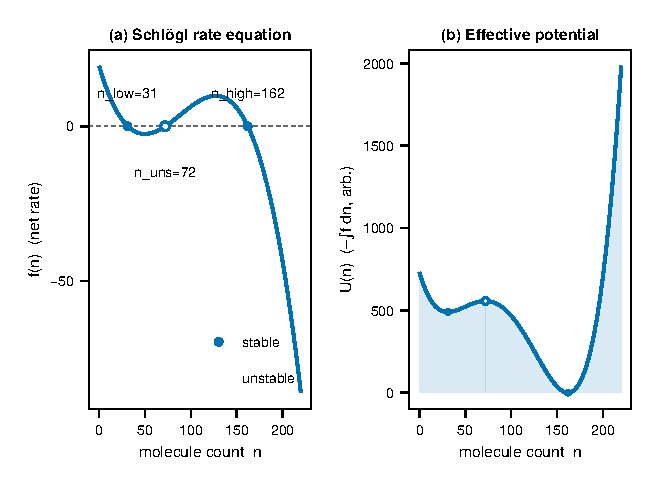
\includegraphics[width=\textwidth]{fig1_schlogl_bistability}
  \caption{Schlögl rate equation $f(n)$ (left) and effective
    potential $U(n) = -\!\int_0^n f(m)\,dm$ (right).
    Stable fixed points at $n_{\mathrm{low}}=31$ and
    $n_{\mathrm{high}}=162$ correspond to the two potential wells.
    The unstable fixed point at $n_{\mathrm{uns}}=72$ is a potential
    barrier.  Parameters: $c_1=0.028$, $c_2=3.2\times10^{-4}$,
    $c_3=19.5$, $c_4=1.0$.}
  \label{fig:schlogl-bistability}
\end{figure}

\paragraph{Benchmark 2a: Markov State Aggregation ($K=2$).}
To isolate the prolongation error, we first test the coarse-only
(MSA) approximation on a $K = 2$ domain with voxel size $h = 1/2$,
diffusion rate $d = D/h^2 = 0.02$.  The initial condition is the
\emph{bistable front}: $(n_1, n_2) = (n_{\mathrm{low}}, n_{\mathrm{high}}) = (31, 162)$.
The coarse variable is $n_c = n_1 + n_2 = 193$.
The direct FSP uses a $(201)^2 = 40{,}401$-state grid ($n_{\max} = 200$)
as ground truth.

\paragraph{Failure of Binomial prolongation.}
The Binomial-$\pi$ prolongation maps $n_c = 193$ to
$\Bin(193, 1/2)$, which peaks at $n_1 = 96$---far from
both stable states.  The TV distance between the Binomial-prolonged
distribution and the direct FSP solution equals
$\TV(\text{Binom-}\pi, \text{FSP}) = 1.000$ at all times
(Figure~\ref{fig:msa-tv-decay}).

\paragraph{Dynamic-$\pi$ prolongation.}
The dynamic-$\pi$ table is computed once from the stationary
distribution of the $K=2$ RDME: $A^\top \pi = 0$, $\sum \pi = 1$
(sparse LU, $1.7\,\mathrm{s}$).  The conditional distribution
$\pi(n_1 \mid n_c = 193)$ is bimodal with peaks near $n_1 = 31$
and $n_1 = 162$ (Figure~\ref{fig:prolongation-failure}), correctly
identifying both stable states.  However, because the stationary
distribution is symmetric under $n_1 \leftrightarrow n_2$, both
modes are assigned equal probability $\approx 0.5$, whereas the
true distribution at $t = 0$ is entirely at $(31, 162)$.
This \emph{symmetry trap} is fundamental: the coarse variable
$n_c$ loses the directionality of the front.

\begin{figure}[ht]
  \centering
  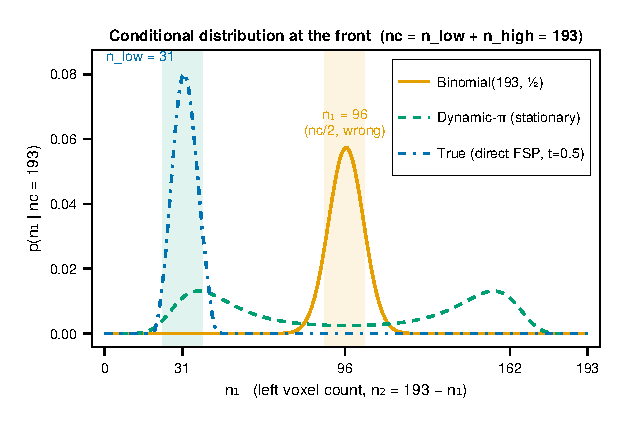
\includegraphics[width=0.75\textwidth]{fig2_prolongation_failure}
  \caption{Conditional distribution $p(n_1 \mid n_c = 193)$ for
    three prolongation methods at $t = 0.5$.
    Binomial($193$, $\frac{1}{2}$) concentrates all mass at the
    wrong location $n_1 = 96$.
    Dynamic-$\pi$ (stationary) correctly identifies both stable
    states at $n_1 \approx 31$ and $n_1 \approx 162$, but assigns
    50\% weight to each (symmetry trap).
    The true conditional (direct FSP) is concentrated near $n_1 = 31$
    since the initial condition has molecules in the low-state voxel.}
  \label{fig:prolongation-failure}
\end{figure}

Figure~\ref{fig:heatmap-comparison} shows the full 2D joint
distribution $p(n_1, n_2)$ at $t = 0.5$.  The Binomial prolongation
places mass at $(96, 97)$ on the anti-diagonal---completely wrong.
Dynamic-$\pi$ prolongation recovers the bimodal structure at
$(31, 162)$ and $(162, 31)$, achieving
$\TV(\text{Dyn-}\pi, \text{FSP}) = 0.798$---a $5\times$ improvement
over Binomial, but not zero due to the symmetry trap.

\begin{figure}[ht]
  \centering
  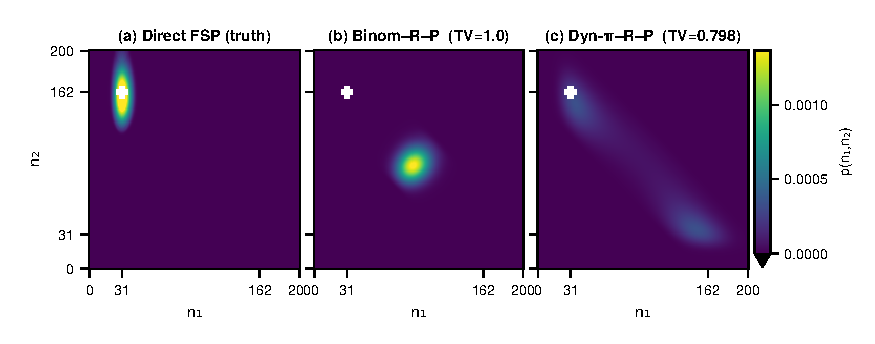
\includegraphics[width=\textwidth]{fig3_heatmap_comparison}
  \caption{Joint fine-level distribution $p(n_1, n_2)$ at $t = 0.5$
    for the $K=2$ Schlögl front IC $(n_1,n_2)=(31,162)$.
    \textbf{(a)} Direct FSP (ground truth): mass concentrated at $(31,162)$.
    \textbf{(b)} Restrict $\to$ Binomial-$\pi$ prolong: wrong location $(96,97)$;
    TV$=1.000$.
    \textbf{(c)} Restrict $\to$ Dynamic-$\pi$ prolong: bimodal at $(31,162)$
    and $(162,31)$; TV$=0.798$.
    White cross marks the initial condition.
    Color scale clipped at 70\% of peak for visibility.}
  \label{fig:heatmap-comparison}
\end{figure}

Figure~\ref{fig:msa-tv-decay} shows the TV evolution over time.
Binomial-$\pi$ maintains TV$\approx 1$ throughout.  Dynamic-$\pi$
starts at TV$= 0.837$ at $t = 0.5$ and decreases toward $0.70$
as the stationary distribution is approached and the symmetry trap
becomes less severe.

\begin{figure}[ht]
  \centering
  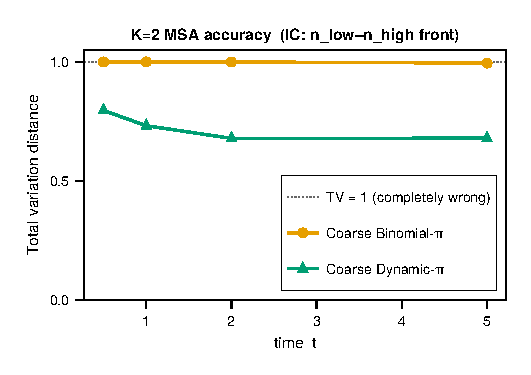
\includegraphics[width=0.5\textwidth]{fig4_msa_tv_decay}
  \caption{TV distance vs.\ direct FSP for the $K=2$ coarse MSA
    methods.  Binomial-$\pi$ is consistently TV$=1$ (completely
    wrong).  Dynamic-$\pi$ achieves TV$\approx 0.80$--$0.70$,
    improving over time as the distribution relaxes toward the
    stationary regime where the symmetric prolongation is more accurate.}
  \label{fig:msa-tv-decay}
\end{figure}

\paragraph{Benchmark 2b: Two-Level V-Cycle ($K=4 \to K=2$).}
With $K = 4$ voxels ($h = 1/4$, $d = 0.08$), a direct FSP at
$n_{\max} = 180$ would require $(181)^4 \approx 1.07 \times 10^9$
states---intractable.  We compare four methods:
(i)~Coarse-only Binomial-$\pi$ ($K=2$ coarse solve, Binom prolong to $K=4$);
(ii)~Coarse-only Dynamic-$\pi$ ($K=2$ coarse solve, Dyn-$\pi$ prolong);
(iii)~V-cycle Binomial-$\pi$ (Algorithm~\ref{alg:vcycle} with Binom correction);
(iv)~V-cycle Dynamic-$\pi$ (Algorithm~\ref{alg:vcycle} with Dyn-$\pi$ correction).

The initial condition is the symmetric front
$(n_{\mathrm{low}}, n_{\mathrm{low}}, n_{\mathrm{high}}, n_{\mathrm{high}}) = (31,31,162,162)$,
where both pairs start at their respective stable fixed points.
Since a direct $K=4$ FSP is intractable, we use two independent
$K=2$ pair FSPs as a proxy ground truth: pair~1 evolves from $(31,31)$,
pair~2 from $(162,162)$.  The TV distance is computed against the
product distribution $p_{\mathrm{GT}}(n_1,n_2,n_3,n_4) = p_1(n_1,n_2)\cdot p_2(n_3,n_4)$.

\begin{figure}[ht]
  \centering
  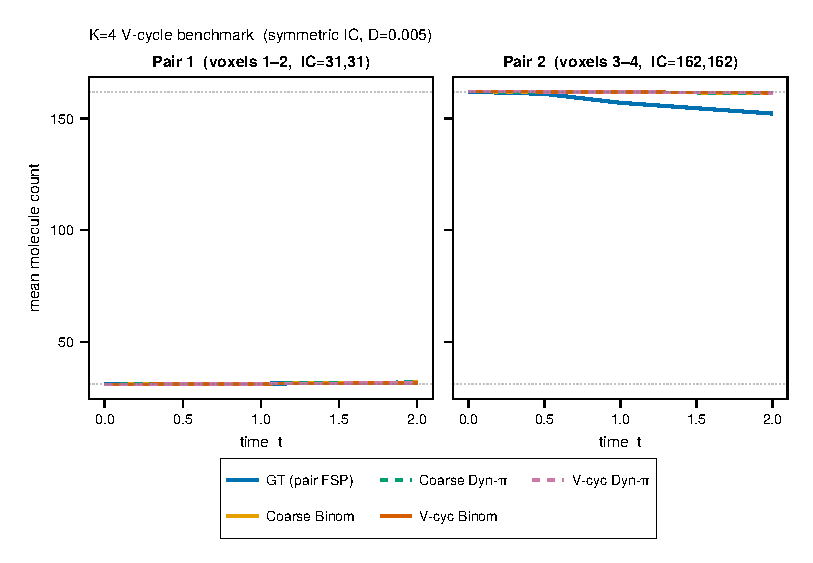
\includegraphics[width=\textwidth]{fig5_vcycle_means}
  \caption{Per-voxel mean molecule counts vs.\ time for the
    $K=4$ V-cycle benchmark (symmetric IC, $D=0.005$).
    All methods track the ground truth (pair FSP, solid blue) closely
    for the mean.  The high TV distances in Figure~\ref{fig:vcycle-accuracy}
    arise from distributional rather than mean errors.}
  \label{fig:vcycle-means}
\end{figure}

\begin{figure}[ht]
  \centering
  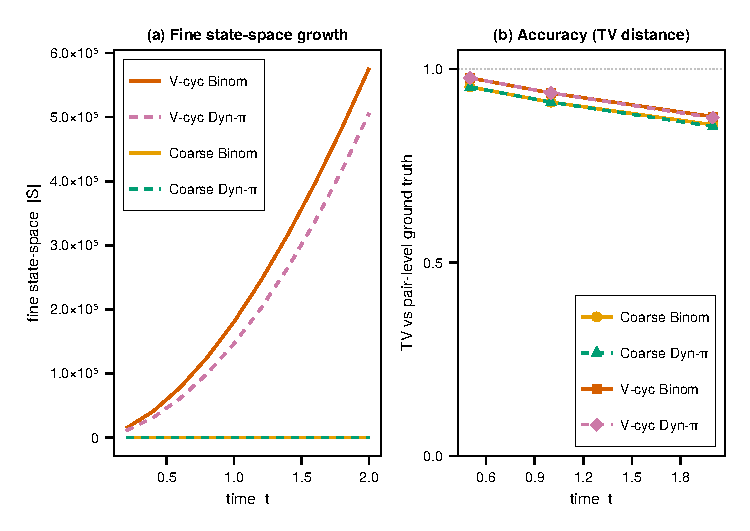
\includegraphics[width=\textwidth]{fig6_vcycle_accuracy}
  \caption{\textbf{(a)} Fine-level state-space size over time.
    V-cycle methods grow to ${\sim}5\times10^5$ fine states by $t=2$;
    coarse-only methods maintain ${\lesssim}10^3$ coarse states.
    \textbf{(b)} TV distance vs.\ pair-level ground truth.
    All four methods produce similar TV values ($0.85$--$0.97$)
    because the error is dominated by inter-pair coupling (the
    independence assumption in the proxy GT) rather than
    prolongation error.  Dynamic-$\pi$ V-cycle runs $5\times$ faster
    than Binomial V-cycle (5.4\,s vs.\ 27.9\,s) with a smaller
    fine state space (506k vs.\ 576k states).}
  \label{fig:vcycle-accuracy}
\end{figure}

Table~\ref{tab:vcycle-tv} summarizes the TV distances and timing.
For this symmetric IC, Binomial-$\pi$ and Dynamic-$\pi$ achieve
nearly identical accuracy because the coarse counts
$n_c^{(1)} = 2 n_{\mathrm{low}} = 62$ and $n_c^{(2)} = 2 n_{\mathrm{high}} = 324$
are both unimodal in the stationary and Binomial prolongations
(both peak at the correct fixed point).  The TV values measure
\emph{inter-pair coupling error} (the product-distribution
approximation) rather than prolongation error.

\begin{table}[ht]
\centering
\caption{K=4 V-cycle benchmark: TV distance vs.\ pair-level
  ground truth and wall-clock timing.  All methods solve from
  $t=0$ to $t_f = 2$ with step size $\Delta t = 0.2$.
  V-cycle methods use pre-smoothing time
  $\tau_{\mathrm{pre}} = 1/(d\,n_{\mathrm{low}}+1) \approx 0.39\,\mathrm{s}$.}
\label{tab:vcycle-tv}
\small
\begin{tabular}{l|ccc|c|c}
\hline
Method & $\TV(t{=}0.5)$ & $\TV(t{=}1)$ & $\TV(t{=}2)$
       & Time (s) & Fine states \\
\hline
Coarse Binom-$\pi$  & 0.954 & 0.915 & 0.856 & 11.2  & $\lesssim 10^3$ \\
Coarse Dyn-$\pi$    & 0.954 & 0.914 & 0.852 &  1.7  & $\lesssim 10^3$ \\
V-cycle Binom-$\pi$ & 0.977 & 0.938 & 0.877 & 27.9  & 576{,}449 \\
V-cycle Dyn-$\pi$   & 0.977 & 0.938 & 0.875 &  5.4  & 506{,}229 \\
\hline
\end{tabular}
\end{table}

\begin{remark}[Symmetric IC and the symmetry trap]
\label{rem:symmetric-ic}
For the symmetric initial condition $(n_{\mathrm{low}}, n_{\mathrm{low}},
n_{\mathrm{high}}, n_{\mathrm{high}})$, both Binomial and Dynamic-$\pi$
prolongation give the same coarse-to-fine mapping (both modes are
unimodal for $n_c = 2n_{\mathrm{low}}$ and $n_c = 2n_{\mathrm{high}}$).
The symmetry trap only manifests for \emph{asymmetric} coarse
states such as $n_c = n_{\mathrm{low}} + n_{\mathrm{high}} = 193$,
as demonstrated in Benchmark~2a.  For applications where all
spatial fronts are at coarse boundaries (i.e.\ the coarse grid
aligns with the front), the symmetric IC benchmark measures the
inter-pair coupling error of the V-cycle architecture
independently of the prolongation operator.
\end{remark}

% =============================================================
\section{Discussion and Outlook}
\label{sec:discussion}
% =============================================================

\paragraph{Dual lumpability as the organizing principle.}
The central contribution of this work is recognizing that the RDME
Markov chain admits lumpability in two independent dimensions:
the molecular-count dimension (fast reactions $\to$ QSS
aggregation) and the spatial dimension (fast diffusion $\to$
voxel merging).  The companion FP-FSP work \cite{Dhumuntarao2024}
operates in the molecular-count dimension; the present multigrid
method operates in the spatial dimension.  Both coarsenings are
instances of the same mathematical operation
(Definition~\ref{def:lumpability}), driven by the same
lumpability parameter (ratio of inter-group to intra-group
transition rates), and require the same bottleneck protection
(Section~\ref{sec:failure-modes}).

A fully adaptive RDME solver would perform both coarsenings
simultaneously: aggregating fast-reaction chains in each voxel
(reducing the per-voxel state space) while merging slow-diffusion
voxel pairs (reducing the number of voxels).  The resulting
two-dimensional coarsening hierarchy acts on the full product
state space $\Znn^{N \times K}$, with each dimension coarsened
independently according to its own lumpability parameter.

\paragraph{Relation to QSS methods.}
Quasi-steady-state (QSS) approximations for the CME \cite{peles}
project out fast species by assuming they reach their conditional
stationary distribution instantaneously.  Our multigrid framework
recovers this limit when $L=1$ and $\tau_{\mathrm{pre}} \to \infty$:
the pre-smoothing step equilibrates the intra-voxel distribution,
and the coarse solve handles only the slow inter-voxel dynamics.
From the lumpability perspective (Section~\ref{sec:lumpability}),
QSS is approximate strong lumpability in the molecular-count
dimension, while our voxel merging is approximate strong
lumpability in the spatial dimension.  The key difference from
classical QSS is that we quantify the approximation error via
$\epsilon_{\mathrm{smooth}}$ and $\epsilon_{kk'}^{(\ell)}$
(Theorem~\ref{thm:vcycle-error} and
Theorem~\ref{thm:approx-lump}), whereas classical QSS has
$O(\epsilon)$ errors without sharp bounds.

\paragraph{Tensor-train methods.}
Tensor-train (TT) decompositions \cite{Kazeev2014} exploit the
same tensor-product structure \eqref{eq:tensor-decomp} to
compress the probability tensor.  TT-cross approximation of the
RDME distribution is an alternative computational approach.  The
multigrid method complements TT methods: while TT reduces storage
by exploiting low-rank structure, multigrid reduces the effective
time-stepping stiffness by hierarchical level decomposition.  A
combined multigrid-TT method is a natural direction for future
work.

\paragraph{RDME vs.\ SSME.}
At very fine spatial resolution (voxel size comparable to the
molecular interaction radius), the RDME becomes inconsistent and
must be replaced by the \emph{spatially continuous master
equation} (SCME) or related formulations \cite{Hellander2012}.
The multigrid framework developed here applies at the RDME level
of description; extending it to continuous-space models is an
open problem.

\paragraph{Higher-order prolongation.}
The binomial prolongation \eqref{eq:prolongation} uses only the
total count $\bar{x}_{ij}$ to reconstruct the within-voxel split.
A higher-order prolongation could incorporate correlations from
the preceding fine-level distribution, analogous to the
\emph{injection} vs.\ \emph{interpolation} prolongation operators
in classical geometric multigrid.

\bibliographystyle{siamplain}
\bibliography{references}

\end{document}
